\begin{frame}{Shakespeare Programming Language}
    
    \begin{columns}

        \begin{column}{.5\hsize}
            \begin{itemize}
                \myitem Karl Hasselström \& Jon Åslund, 2001
                \myitem Program w SPL wygląda jak szekspirowska sztuka
                \myitem Postacie to zmienne
                \myitem Wielkość zmiennej zależy wykładniczo od liczby przypisanych do niej komplementów lub przywar
            \end{itemize}
        \end{column}

        \begin{column}{.5\hsize}
            \begin{figure}
                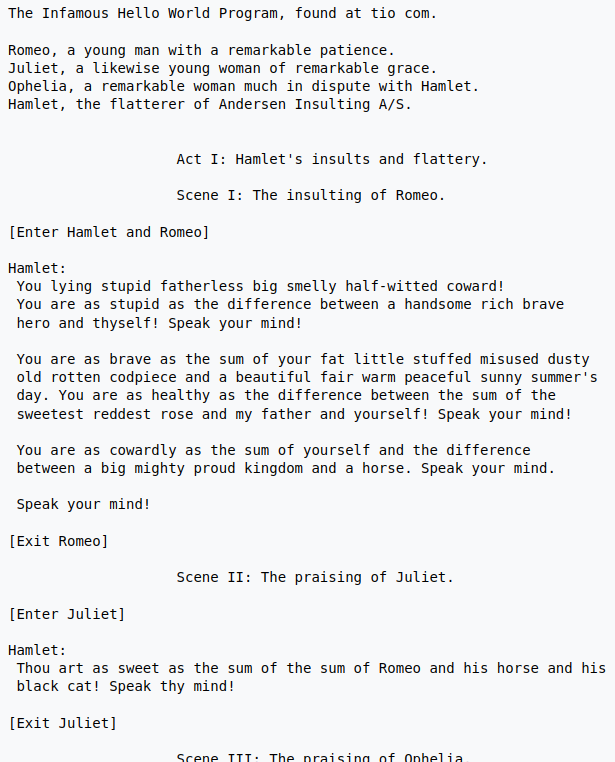
\includegraphics[height=6.3cm]{figures/spl.png}
                \caption*{\footnotesize Fragment sztuki ,,Hello World'' {\color{blue} \hyperlink{frame:przypisy}{(5)}}}
            \end{figure}
        \end{column}

    \end{columns}

\end{frame}
